\section{Experiments}
\label{sec:experiments}
    H-SFP is evaluated on CIFAR-10/100~\cite{krizhevsky2009learning}, HAM10000~\cite{tschandl2018ham10000}, ImageNet-1K~\cite{5206848}, and ISIC-2018~\cite{8363547} against FedAvg, FedProx, FedProto, HierFL, SplitFed, and HSFL baselines. HSFL serves as our primary architectural baseline. FedAvg and FedProx are included to benchmark standard and regularized parameter-based synchronization. We select FedProto and FedGen to compare our generative synthesis against state-of-the-art prototype-based and data-free distillation methods. To address system heterogeneity, we compare against SplitFed and HeteroSFL. HierFL and HSFL serve as our primary architectural baselines to isolate the specific benefits of our prototype-driven coordination within hierarchical topologies. Our setup comprises 200 clients, partitioned across 10 edge servers, for all hierarchical methods. All models use the Adam optimizer ($lr=1e-4$), and we report classification accuracy, segmentation performance, communication overhead, and client-side RAM usage. Specific hyperparameters, the full experimental setup, and additional results are detailed in the Appendix~D.

\subsection{Main Results: Model Performance}
\begin{table}[htbp]
    \centering
    \caption{Accuracy (\%) on CIFAR-10 and CIFAR-100 under IID and non-IID (Dirichlet) settings across 200 distributed devices. Results are averaged over 5 independent runs, showing mean $\pm$ std. (A), (B), and (C) represent client-edge ($I_c$) and edge-cloud ($I_e$) aggregation intervals of (5, 10), (10, 20), and (25, 50) local epochs, respectively. \textbf{Bold} indicates best federated performance; \underline{underline} indicates second-best.}
    \label{tab:cifar_accuracy}
    \resizebox{\textwidth}{!}{
    \begin{tabular}{l|ccc|ccc}
        \toprule
        \multirow{2}{*}{\textbf{Method}} &
        \multicolumn{3}{c|}{\textbf{CIFAR-10}} &
        \multicolumn{3}{c}{\textbf{CIFAR-100}} \\
        \cmidrule{2-7}
        & \textbf{IID} & $dir(0.3)$ & $dir(0.7)$ & \textbf{IID} & $dir(0.3)$ & $dir(0.7)$ \\
        \midrule\midrule
        \textbf{Centralized} & 94.20 {\scriptsize $\pm$ 0.35} & N/A & N/A & 75.60 {\scriptsize $\pm$ 0.45} & N/A & N/A \\
        \midrule
        FedAvg & 57.25 {\scriptsize $\pm$ 1.24} & 12.15 {\scriptsize $\pm$ 2.10} & 23.60 {\scriptsize $\pm$ 1.85} & 48.85 {\scriptsize $\pm$ 1.40} & 2.10 {\scriptsize $\pm$ 0.85} & 5.40 {\scriptsize $\pm$ 1.15} \\
        FedSGD & 18.80 {\scriptsize $\pm$ 1.10} & 5.80 {\scriptsize $\pm$ 0.95} & 6.40 {\scriptsize $\pm$ 0.80} & 10.75 {\scriptsize $\pm$ 0.90} & 1.80 {\scriptsize $\pm$ 0.40} & 4.35 {\scriptsize $\pm$ 0.65} \\
        FedNova & 23.50 {\scriptsize $\pm$ 1.15} & 14.20 {\scriptsize $\pm$ 1.50} & 18.35 {\scriptsize $\pm$ 1.45} & 50.24 {\scriptsize $\pm$ 1.35} & 3.15 {\scriptsize $\pm$ 0.75} & 6.80 {\scriptsize $\pm$ 0.95} \\
        FedProx & 58.25 {\scriptsize $\pm$ 1.20} & 16.50 {\scriptsize $\pm$ 1.80} & 25.40 {\scriptsize $\pm$ 1.60} & 52.75 {\scriptsize $\pm$ 1.25} & 4.05 {\scriptsize $\pm$ 0.85} & 7.20 {\scriptsize $\pm$ 1.10} \\
        FedProto & 55.10 {\scriptsize $\pm$ 1.05} & 38.50 {\scriptsize $\pm$ 1.45} & 45.20 {\scriptsize $\pm$ 1.30} & 46.50 {\scriptsize $\pm$ 1.15} & 6.50 {\scriptsize $\pm$ 0.95} & 8.80 {\scriptsize $\pm$ 1.05} \\
        HierFL & 62.50 {\scriptsize $\pm$ 1.30} & 13.10 {\scriptsize $\pm$ 1.90} & 23.60 {\scriptsize $\pm$ 1.75} & 30.15 {\scriptsize $\pm$ 1.45} & 1.95 {\scriptsize $\pm$ 0.60} & 4.78 {\scriptsize $\pm$ 0.85} \\
        SplitFed & 61.85 {\scriptsize $\pm$ 1.25} & 31.20 {\scriptsize $\pm$ 1.65} & 39.95 {\scriptsize $\pm$ 1.40} & 35.00 {\scriptsize $\pm$ 1.30} & 4.15 {\scriptsize $\pm$ 0.80} & 7.05 {\scriptsize $\pm$ 1.00} \\
        HeteroSFL & 63.45 {\scriptsize $\pm$ 1.10} & 33.80 {\scriptsize $\pm$ 1.45} & 42.60 {\scriptsize $\pm$ 1.30} & 41.50 {\scriptsize $\pm$ 1.25} & 5.45 {\scriptsize $\pm$ 0.70} & 8.20 {\scriptsize $\pm$ 0.95} \\
        FedGen & 59.80 {\scriptsize $\pm$ 1.10} & 37.90 {\scriptsize $\pm$ 1.50} & 46.10 {\scriptsize $\pm$ 1.25} & 51.20 {\scriptsize $\pm$ 1.25} & 6.70 {\scriptsize $\pm$ 0.85} & 9.15 {\scriptsize $\pm$ 1.10} \\
        FedDF & 61.50 {\scriptsize $\pm$ 1.15} & 32.00 {\scriptsize $\pm$ 1.60} & 40.50 {\scriptsize $\pm$ 1.35} & 53.10 {\scriptsize $\pm$ 1.20} & 4.50 {\scriptsize $\pm$ 0.70} & 7.80 {\scriptsize $\pm$ 1.05} \\
        \midrule
        HSFL (A) & 51.35 {\scriptsize $\pm$ 1.10} & 17.80 {\scriptsize $\pm$ 1.75} & 26.54 {\scriptsize $\pm$ 1.50} & 35.47 {\scriptsize $\pm$ 1.35} & 5.10 {\scriptsize $\pm$ 0.80} & 8.25 {\scriptsize $\pm$ 1.15} \\
        HSFL (B) & 50.80 {\scriptsize $\pm$ 1.05} & 17.15 {\scriptsize $\pm$ 1.65} & 25.90 {\scriptsize $\pm$ 1.45} & 33.58 {\scriptsize $\pm$ 1.30} & 4.80 {\scriptsize $\pm$ 0.75} & 7.65 {\scriptsize $\pm$ 1.10} \\
        HSFL (C) & 49.18 {\scriptsize $\pm$ 1.15} & 16.90 {\scriptsize $\pm$ 1.70} & 25.40 {\scriptsize $\pm$ 1.55} & 32.65 {\scriptsize $\pm$ 1.40} & 4.10 {\scriptsize $\pm$ 0.85} & 6.95 {\scriptsize $\pm$ 1.05} \\
        \midrule
        \textbf{Ours (A)} & \textbf{67.44 {\scriptsize $\pm$ 0.85}} & \textbf{40.15 {\scriptsize $\pm$ 1.25}} & \textbf{48.85 {\scriptsize $\pm$ 1.10}} & \textbf{55.10 {\scriptsize $\pm$ 0.95}} & \textbf{7.15 {\scriptsize $\pm$ 0.65}} & \textbf{10.48 {\scriptsize $\pm$ 0.85}} \\
        \textbf{Ours (B)} & \underline{66.80 {\scriptsize $\pm$ 0.80}} & \underline{39.80 {\scriptsize $\pm$ 1.20}} & \underline{48.15 {\scriptsize $\pm$ 1.05}} & \underline{54.25 {\scriptsize $\pm$ 0.90}} & \underline{6.80 {\scriptsize $\pm$ 0.60}} & \underline{9.95 {\scriptsize $\pm$ 0.80}} \\
        \textbf{Ours (C)} & 65.44 {\scriptsize $\pm$ 0.90} & 39.10 {\scriptsize $\pm$ 1.30} & 47.50 {\scriptsize $\pm$ 1.15} & 53.65 {\scriptsize $\pm$ 1.00} & 6.15 {\scriptsize $\pm$ 0.70} & 9.05 {\scriptsize $\pm$ 0.90} \\
        \bottomrule
    \end{tabular}
    }
\end{table}
\begin{table}[t]
    \centering
    \caption{Accuracy (\%) on HAM10000 and ImageNet-1K under different backbones and data distributions. Results are averaged over 5 runs across 200 clients (mean $\pm$ std). (A), (B), and (C) denote different client-edge and edge-cloud aggregation intervals. \textbf{Bold} and \underline{underline} indicate the best and second-best federated results, respectively.}
        \label{tab:complex_accuracy}
    \resizebox{\textwidth}{!}{
    \begin{tabular}{l|ccc|ccc}
        \toprule
        \multirow{2}{*}{\textbf{Method}} & \multicolumn{3}{c|}{\textbf{HAM10000}} & \multicolumn{3}{c}{\textbf{ImageNet-1K}} \\ \cmidrule{2-7} 
        & \textbf{\begin{tabular}[c]{@{}c@{}}ResNet-50\\ (IID)\end{tabular}} & \textbf{\begin{tabular}[c]{@{}c@{}}VGG-16\\ (IID)\end{tabular}} & \textbf{\begin{tabular}[c]{@{}c@{}}ResNet-50\\ ($dir(0.7)$)\end{tabular}} & \textbf{\begin{tabular}[c]{@{}c@{}}ResNet-50 \\ (IID)\end{tabular}} & \textbf{\begin{tabular}[c]{@{}c@{}}VGG-16 \\ (IID)\end{tabular}} & \textbf{\begin{tabular}[c]{@{}c@{}}ResNet-50 \\ ($dir(0.7)$)\end{tabular}} \\
        \midrule\midrule
        \textbf{Centralized} & 86.40 {\scriptsize $\pm$ 0.60} & 84.20 {\scriptsize $\pm$ 0.55} & N/A & 75.8 {\scriptsize $\pm$ 0.2} & 72.4 {\scriptsize $\pm$ 0.3} & N/A \\
        \midrule
        FedAvg & 68.28 {\scriptsize $\pm$ 1.45} & 65.15 {\scriptsize $\pm$ 1.50} & 13.45 {\scriptsize $\pm$ 1.65} & 23.1 {\scriptsize $\pm$ 1.4} & 21.4 {\scriptsize $\pm$ 1.5} & 11.2 {\scriptsize $\pm$ 1.7} \\
        FedSGD & 25.85 {\scriptsize $\pm$ 1.20} & 22.40 {\scriptsize $\pm$ 1.10} & 6.34 {\scriptsize $\pm$ 1.05} & 12.5 {\scriptsize $\pm$ 1.1} & 10.2 {\scriptsize $\pm$ 1.2} & 5.4 {\scriptsize $\pm$ 1.1} \\
        FedNova & 69.60 {\scriptsize $\pm$ 1.35} & 67.30 {\scriptsize $\pm$ 1.45} & 14.35 {\scriptsize $\pm$ 1.50} & 23.8 {\scriptsize $\pm$ 1.3} & 22.1 {\scriptsize $\pm$ 1.4} & 12.5 {\scriptsize $\pm$ 1.6} \\
        FedProx & 71.15 {\scriptsize $\pm$ 1.30} & 68.85 {\scriptsize $\pm$ 1.40} & 15.45 {\scriptsize $\pm$ 1.55} & 24.1 {\scriptsize $\pm$ 1.3} & 22.5 {\scriptsize $\pm$ 1.4} & 13.8 {\scriptsize $\pm$ 1.6} \\
        FedProto & 67.20 {\scriptsize $\pm$ 1.25} & 64.50 {\scriptsize $\pm$ 1.35} & 35.00 {\scriptsize $\pm$ 1.40} & 25.2 {\scriptsize $\pm$ 1.2} & 23.8 {\scriptsize $\pm$ 1.3} & 18.5 {\scriptsize $\pm$ 1.4} \\
        HierFL & 69.50 {\scriptsize $\pm$ 1.25} & 67.10 {\scriptsize $\pm$ 1.30} & 22.40 {\scriptsize $\pm$ 1.55} & 24.5 {\scriptsize $\pm$ 1.2} & 22.8 {\scriptsize $\pm$ 1.3} & 13.8 {\scriptsize $\pm$ 1.5} \\
        SplitFed & 65.78 {\scriptsize $\pm$ 1.35} & 62.90 {\scriptsize $\pm$ 1.40} & 25.15 {\scriptsize $\pm$ 1.45} & 25.5 {\scriptsize $\pm$ 1.1} & 23.4 {\scriptsize $\pm$ 1.2} & 14.1 {\scriptsize $\pm$ 1.5} \\
        HeteroSFL & 67.10 {\scriptsize $\pm$ 1.20} & 64.80 {\scriptsize $\pm$ 1.25} & 28.50 {\scriptsize $\pm$ 1.35} & 26.3 {\scriptsize $\pm$ 0.8} & 24.2 {\scriptsize $\pm$ 0.9} & 16.2 {\scriptsize $\pm$ 1.2} \\
        FedGen & 72.50 {\scriptsize $\pm$ 1.15} & 69.40 {\scriptsize $\pm$ 1.20} & 35.80 {\scriptsize $\pm$ 1.30} & 26.8 {\scriptsize $\pm$ 1.0} & 24.5 {\scriptsize $\pm$ 1.1} & 19.3 {\scriptsize $\pm$ 1.3} \\
        FedDF & 73.10 {\scriptsize $\pm$ 1.20} & 70.20 {\scriptsize $\pm$ 1.30} & 27.80 {\scriptsize $\pm$ 1.45} & 25.9 {\scriptsize $\pm$ 1.1} & 23.9 {\scriptsize $\pm$ 1.2} & 15.6 {\scriptsize $\pm$ 1.4} \\
        \midrule
        HSFL (A) & 68.82 {\scriptsize $\pm$ 1.25} & 66.15 {\scriptsize $\pm$ 1.35} & 30.45 {\scriptsize $\pm$ 1.40} & 24.6 {\scriptsize $\pm$ 0.9} & 22.5 {\scriptsize $\pm$ 1.0} & 14.8 {\scriptsize $\pm$ 1.1} \\
        HSFL (B) & 67.74 {\scriptsize $\pm$ 1.20} & 65.20 {\scriptsize $\pm$ 1.25} & 28.83 {\scriptsize $\pm$ 1.35} & 24.1 {\scriptsize $\pm$ 0.9} & 22.1 {\scriptsize $\pm$ 1.0} & 13.9 {\scriptsize $\pm$ 1.2} \\
        HSFL (C) & 66.98 {\scriptsize $\pm$ 1.30} & 64.50 {\scriptsize $\pm$ 1.30} & 27.95 {\scriptsize $\pm$ 1.45} & 23.5 {\scriptsize $\pm$ 1.0} & 21.6 {\scriptsize $\pm$ 1.1} & 13.1 {\scriptsize $\pm$ 1.2} \\
        \midrule
        \textbf{Ours (A)} & \textbf{80.86 {\scriptsize $\pm$ 0.75}} & \textbf{78.45 {\scriptsize $\pm$ 0.80}} & \textbf{37.50 {\scriptsize $\pm$ 1.05}} & \textbf{27.9 {\scriptsize $\pm$ 0.3}} & \textbf{25.3 {\scriptsize $\pm$ 0.4}} & \textbf{22.4 {\scriptsize $\pm$ 0.6}} \\
        \textbf{Ours (B)} & \underline{79.96 {\scriptsize $\pm$ 0.70}} & \underline{77.50 {\scriptsize $\pm$ 0.75}} & \underline{36.90 {\scriptsize $\pm$ 1.00}} & \underline{27.4 {\scriptsize $\pm$ 0.4}} & \underline{24.8 {\scriptsize $\pm$ 0.5}} & \underline{21.8 {\scriptsize $\pm$ 0.7}} \\
        \textbf{Ours (C)} & 79.15 {\scriptsize $\pm$ 0.80} & 76.80 {\scriptsize $\pm$ 0.85} & 36.15 {\scriptsize $\pm$ 1.15} & 26.8 {\scriptsize $\pm$ 0.5} & 24.2 {\scriptsize $\pm$ 0.6} & 21.1 {\scriptsize $\pm$ 0.8} \\
        \bottomrule
    \end{tabular}
    }
\end{table}
\begin{table}[htbp]
    \centering
    \caption{Segmentation performance on the ISIC-2018 dataset using a ResNet50-UNet backbone. All models were trained under a strict constraint of 200 communication rounds across 200 distributed edge devices. \textbf{Bold} indicates the best federated performance, and \underline{underline} indicates the second-best.}
    \label{tab:segmentation_results}
    \begin{tabular}{l|c c c}
        \toprule
        \textbf{Method} & \textbf{IoU (\%)} $\uparrow$ & \textbf{DICE (\%)} $\uparrow$ & \textbf{Training Time (h)} $\downarrow$\\ 
        \midrule\midrule
        \textbf{Centralized} & 78.5 {\scriptsize $\pm$ 0.4} & 86.2 {\scriptsize $\pm$ 0.3} & 5.2 {\scriptsize $\pm$ 0.1} \\
        \midrule
        FedAvg          & 48.7 {\scriptsize $\pm$ 1.2} & 64.2 {\scriptsize $\pm$ 1.5} & 28.5 {\scriptsize $\pm$ 0.8} \\ 
        HierFL          & 51.2 {\scriptsize $\pm$ 1.1} & 66.3 {\scriptsize $\pm$ 1.3} & 24.3 {\scriptsize $\pm$ 0.7} \\
        SplitFed        & 53.8 {\scriptsize $\pm$ 0.9} & 68.1 {\scriptsize $\pm$ 1.1} & 72.4 {\scriptsize $\pm$ 1.6} \\
        HeteroSFL       & 56.4 {\scriptsize $\pm$ 0.7} & 70.5 {\scriptsize $\pm$ 0.8} & 45.8 {\scriptsize $\pm$ 1.2} \\
        HSFL (A)        & \underline{62.1 {\scriptsize $\pm$ 0.8}} & \underline{74.8 {\scriptsize $\pm$ 0.9}} & \underline{14.5 {\scriptsize $\pm$ 0.5}} \\
        \midrule
        \textbf{Ours (A)} & \textbf{68.3 {\scriptsize $\pm$ 0.5}} & \textbf{79.5 {\scriptsize $\pm$ 0.4}} & \textbf{6.8 {\scriptsize $\pm$ 0.2}} \\ 
        \bottomrule
    \end{tabular}
\end{table}

\Cref{tab:cifar_accuracy,tab:complex_accuracy} summarize the classification accuracy across varying datasets, backbones, and statistical distributions. Across all configurations, our proposed H-SFP framework consistently yields the highest performance.

\noindent\textbf{Mitigating severe client drift.} H-SFP shows significant resilience in highly skewed non-IID scenarios. As shown in \Cref{tab:cifar_accuracy}, standard aggregation methods such as FedAvg exhibit a sharp performance drop under extreme data heterogeneity, falling to 12.15\% on CIFAR-10 ($dir(0.3)$). H-SFP (A) effectively mitigates client drift, achieving 40.15\% and outperforming specialized state-of-the-art methods, including FedProto (38.50\%) and FedGen (37.90\%). This confirms that synthesizing global prototypes at the edge and cloud tiers provides a stronger regularizing effect than flat architectural baselines. Furthermore, the varying aggregation intervals (A, B, C) indicate a direct correlation between edge-cloud synchronization frequency and final accuracy.

\noindent\textbf{Scaling to large-scale vision tasks.} To verify that our feature synthesis does not destroy high-rank semantic information, we extended our evaluation to HAM10000 and ImageNet-1K (\Cref{tab:complex_accuracy}). Under a strict 200-round budget across 200 devices, H-SFP (A) achieves 80.86\% on HAM10000 (IID, ResNet-50), closely trailing the unconstrained Centralized Oracle (86.40\%). On ImageNet-1K, H-SFP (A) reaches 27.9\%, outperforming advanced baselines including HeteroSFL (26.3\%) and SplitFed (25.5\%). This demonstrates that transmitting lightweight Gaussian statistics is sufficient to preserve the complex feature manifolds required for standard ResNet and VGG backbones.

\noindent\textbf{Application to dense medical segmentation.} We further evaluate the framework's versatility on the ISIC-2018 skin lesion segmentation task depicted in \Cref{tab:segmentation_results}. Dense prediction tasks expose the primary vulnerability of split learning: transmitting high-dimensional spatial feature maps creates severe communication bottlenecks. Consequently, SplitFed requires 72.4 hours to reach 53.8\% IoU. While weight-averaging methods like FedAvg complete training faster (28.5 hours), they stall at 48.7\% IoU due to unmitigated client drift. H-SFP addresses this bottleneck directly by synthesizing the bottleneck features for the cloud-based decoder rather than transmitting raw activations. As a result, H-SFP achieves $68.3\%$ IoU and $79.5\%$ DICE in only $6.8$ hours, delivering a 10$\times$ training speedup over SplitFed and a 19.6\% absolute IoU improvement over FedAvg.

\subsection{Analysis of Communication Overhead}
\begin{figure}[t]
    \centering
    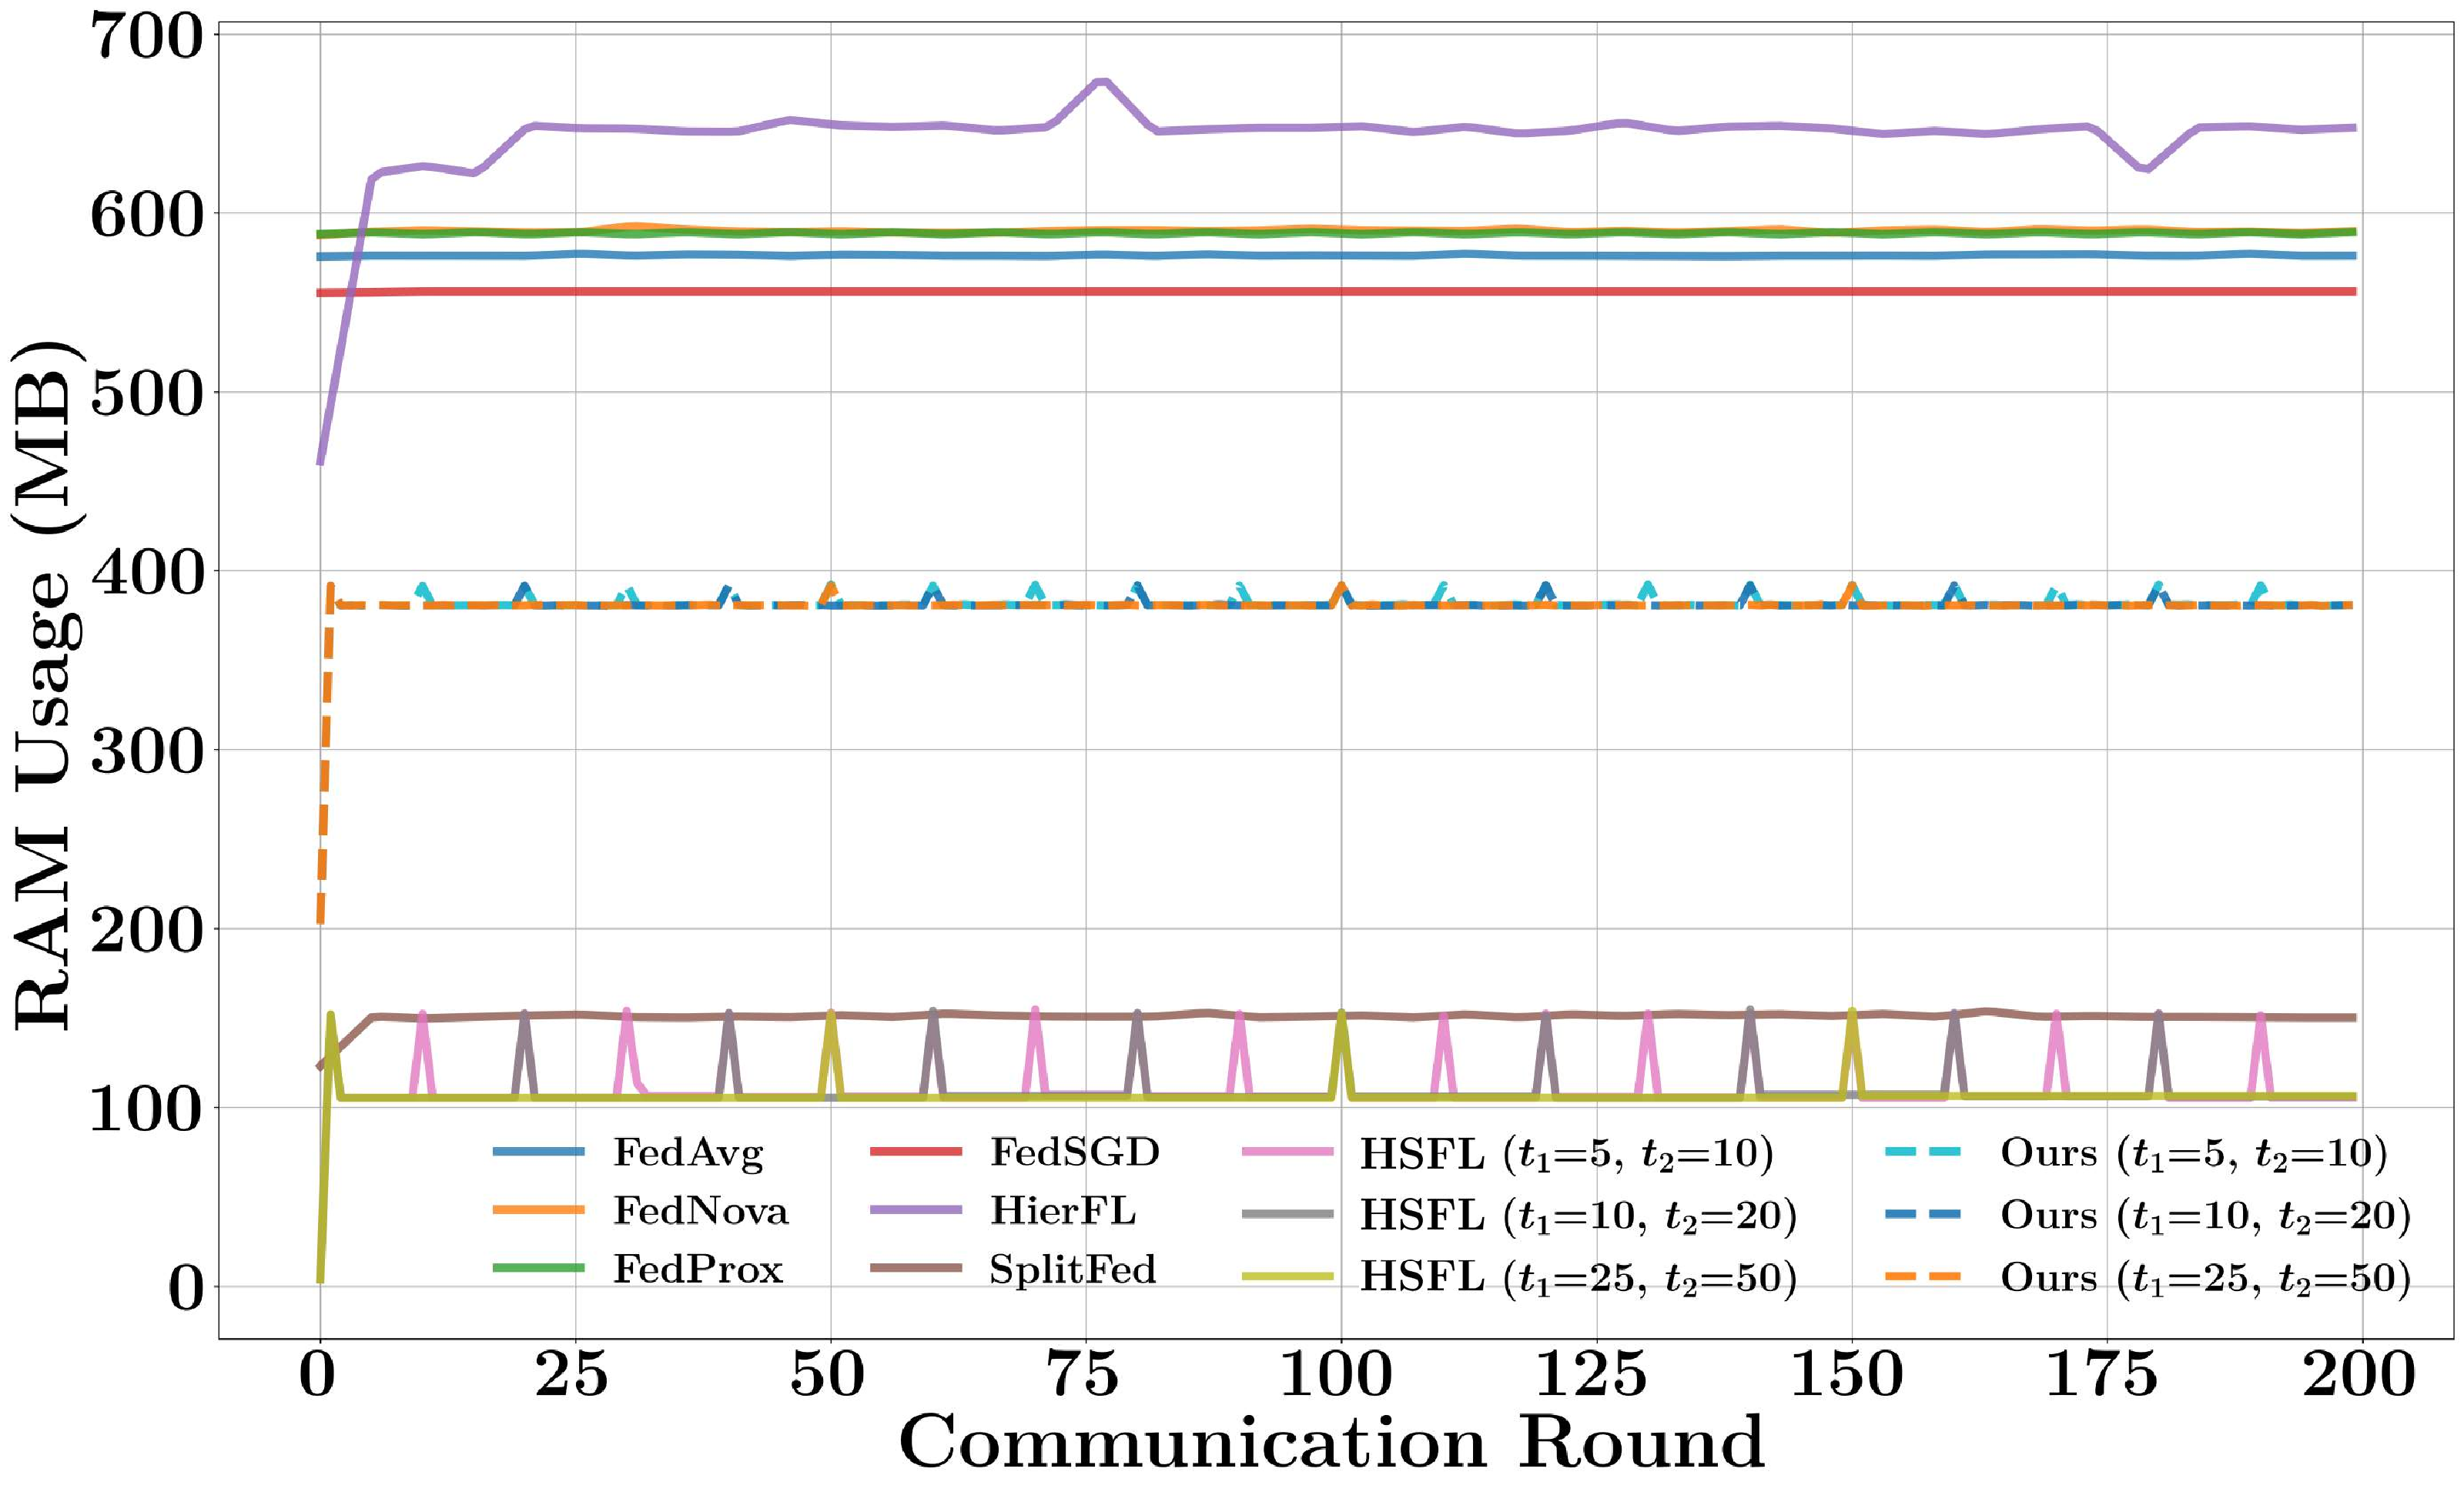
\includegraphics[width=0.8\linewidth]{Figures/cifar_client_gpu_ram_list_comparison.pdf}
    \caption{Client-side RAM usage (MB) over 200 rounds. The chart contrasts the high, stable memory cost of full-model methods ($\sim$600 MB) with the low, sub-100 MB cost of split-learning methods (SplitFed, HSFL, and Ours).}
    \label{fig:computation}
\end{figure}
\begin{figure}[t]
    \centering
    % --- LEFT PLOT: Total Overhead (Log Scale) ---
    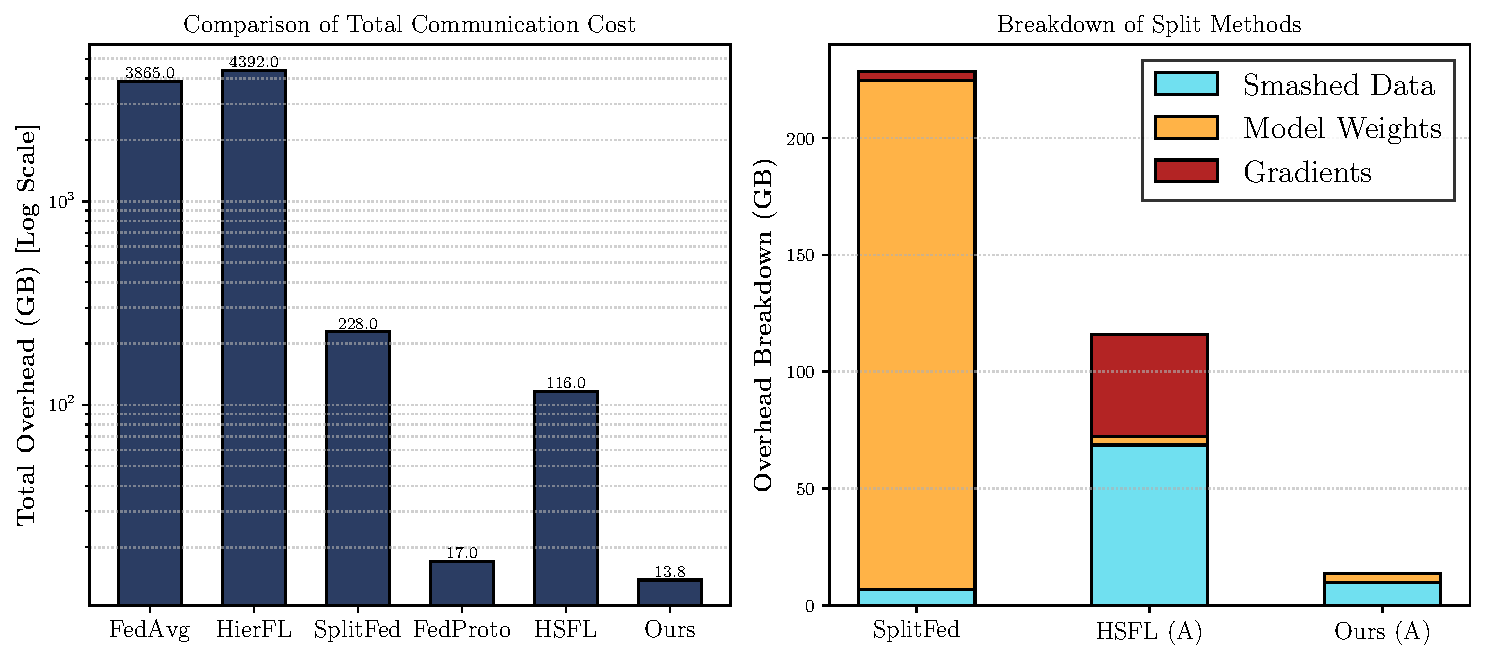
\includegraphics[width=0.8\linewidth]{Figures/communication_overhead.pdf}
    \caption{Communication overhead analysis on CIFAR-100 over $200$ rounds. \textbf{(Left)} Total communication cost across all methods plotted on a logarithmic scale. H-SFP (ours) reduces the total overhead by over $350$$\times$ compared to standard FedAvg. \textbf{(Right)} A detailed breakdown of the communication components for the split-learning baselines. H-SFP's extreme efficiency stems from replacing high-dimensional smashed data with lightweight statistics and eliminating the need to transmit gradients.}
    \label{fig:comm_overhead}
\end{figure}
\Cref{fig:comm_overhead} provides a detailed breakdown of the communication overhead, quantifying the primary advantage of H-SFP. As shown, traditional FL methods like FedAvg are prohibitively expensive ($\sim$3,865 GB) due to full model transfers, and HierFL incurs even higher costs (4,392.44 GB). While hybrid methods such as HSFL (113.12 GB) and prototype-based FedProto ($17.25$ GB) offer significant savings, our H-SFP framework yields the most dramatic reduction. Specifically, our most efficient configuration (Ours (C)) requires only 10.94 GB. This represents a 353$\times$ reduction compared to FedAvg, a 10.4$\times$ reduction over the HSFL baseline, and a $1.58$$\times$ improvement over the strong FedProto baseline. These gains are directly attributable to our novel architecture: H-SFP eliminates the need for gradient backpropagation (which consumes $43.47$ GB in HSFL) and replaces the continuous transfer of raw activations ($54.93$ GB in HSFL) with lightweight feature statistics (9.77 GB), thereby effectively resolving the communication bottleneck.

To better understand the communication savings of H-SFP, we compare its communication complexity with that of standard FSL. In FSL, clients transmit intermediate activations during the forward pass and receive corresponding gradients during the backward pass. As a result, the communication cost per synchronization round scales linearly with the local batch size $B$ and the intermediate feature dimension $d$, $\text{FSL Communication} = \mathcal{O}(B \cdot d)$.
In contrast, H-SFP severs the cross-tier optimization graph, eliminating the need for sample-wise activation and gradient exchanges. Instead, clients in our framework compute and transmit only lightweight statistical moments (e.g., mean and variance) for each class present in their local data. Therefore, the communication overhead scales solely with the number of unique classes $C$ and the feature dimension $d$, $\text{H-SFP Communication} = \mathcal{O}(C \cdot d)$.
In typical distributed learning scenarios, the local batch size is significantly larger than the number of unique classes ($B \gg C$). Furthermore, because H-SFP utilizes these statistical moments for generative synthesis at the upper tiers, it completely circumvents the backward-pass communication phase required by FSL. This fundamental theoretical shift from sample-dependent $\mathcal{O}(B \cdot d)$ complexity to class-dependent $\mathcal{O}(C \cdot d)$ complexity provides the mathematical underpinning for the massive communication savings demonstrated in our empirical results.
\subsection{Analysis of Client-Side Memory Cost}
\Cref{fig:computation} reveals a stark divide: traditional, full-model methods (e.g., FedAvg) require a stable $\sim$600~MB of RAM to load the \textit{entire} model. In contrast, our H-SFP framework and other split-learning methods consume well under 100 MB. This dramatic reduction is due to H-SFP clients managing only the lightweight initial segment ($W_c$). This result confirms that ours is highly practical for resource-constrained clients for whom standard FL is infeasible.

\subsection{Scalability Test}
\begin{table}[!ht]
    \centering
    \caption{Accuracy (\%) on CIFAR-100 and ImageNet-1K under the IID scenario with varying client cohort sizes.
    % The total dataset size is kept fixed to assess robustness to data sparsity. 
    Results are averaged over 5 independent runs (mean $\pm$ std). (A), (B), and (C) represent client-edge and edge-cloud aggregation intervals. \textbf{Bold} indicates the best federated performance, and \underline{underline} indicates the second-best.}
    \label{tab:main_robustness_sparsity}
    \resizebox{\textwidth}{!}{
    \begin{tabular}{l cccc cccc}
        \toprule
        \multirow{2}{*}{\textbf{Method}} & 
        \multicolumn{4}{c}{\textbf{CIFAR-100}} & 
        \multicolumn{4}{c}{\textbf{ImageNet-1K}} \\ 
        \cmidrule(lr){2-5} \cmidrule(lr){6-9}
        & \textbf{200} & \textbf{100} & \textbf{50} & \textbf{20} & \textbf{200} & \textbf{100} & \textbf{50} & \textbf{20} \\
        \midrule
        \midrule
        FedAvg & 48.85 {\scriptsize $\pm$ 1.40} & 53.20 {\scriptsize $\pm$ 1.25} & 57.10 {\scriptsize $\pm$ 1.10} & 60.50 {\scriptsize $\pm$ 0.90} & 23.1 {\scriptsize $\pm$ 1.4} & 31.4 {\scriptsize $\pm$ 1.2} & 42.5 {\scriptsize $\pm$ 1.1} & 53.2 {\scriptsize $\pm$ 0.9} \\
        FedSGD & 10.75 {\scriptsize $\pm$ 0.90} & 13.10 {\scriptsize $\pm$ 0.85} & 15.80 {\scriptsize $\pm$ 0.80} & 17.90 {\scriptsize $\pm$ 0.75} & 12.5 {\scriptsize $\pm$ 1.1} & 15.6 {\scriptsize $\pm$ 1.0} & 21.4 {\scriptsize $\pm$ 0.9} & 28.5 {\scriptsize $\pm$ 0.8} \\
        FedNova & 50.24 {\scriptsize $\pm$ 1.35} & 54.80 {\scriptsize $\pm$ 1.20} & 58.90 {\scriptsize $\pm$ 1.05} & 61.70 {\scriptsize $\pm$ 0.85} & 23.8 {\scriptsize $\pm$ 1.3} & 32.5 {\scriptsize $\pm$ 1.2} & 43.8 {\scriptsize $\pm$ 1.0} & 55.1 {\scriptsize $\pm$ 0.9} \\
        FedProx & 52.75 {\scriptsize $\pm$ 1.25} & 57.00 {\scriptsize $\pm$ 1.15} & 60.90 {\scriptsize $\pm$ 1.00} & 63.80 {\scriptsize $\pm$ 0.85} & 24.1 {\scriptsize $\pm$ 1.3} & 32.8 {\scriptsize $\pm$ 1.1} & 44.2 {\scriptsize $\pm$ 1.0} & 55.8 {\scriptsize $\pm$ 0.8} \\
        FedProto & 49.50 {\scriptsize $\pm$ 1.15} & 53.80 {\scriptsize $\pm$ 1.05} & 57.90 {\scriptsize $\pm$ 0.95} & 61.20 {\scriptsize $\pm$ 0.80} & 25.2 {\scriptsize $\pm$ 1.2} & 34.5 {\scriptsize $\pm$ 1.1} & 46.1 {\scriptsize $\pm$ 0.9} & 57.5 {\scriptsize $\pm$ 0.8} \\
        HierFL & 50.15 {\scriptsize $\pm$ 1.30} & 54.50 {\scriptsize $\pm$ 1.15} & 58.40 {\scriptsize $\pm$ 1.05} & 61.80 {\scriptsize $\pm$ 0.90} & 24.5 {\scriptsize $\pm$ 1.2} & 33.6 {\scriptsize $\pm$ 1.1} & 45.4 {\scriptsize $\pm$ 1.0} & 56.7 {\scriptsize $\pm$ 0.8} \\
        SplitFed & 51.00 {\scriptsize $\pm$ 1.20} & 55.40 {\scriptsize $\pm$ 1.10} & 59.30 {\scriptsize $\pm$ 0.95} & 62.50 {\scriptsize $\pm$ 0.85} & 25.5 {\scriptsize $\pm$ 1.1} & 34.8 {\scriptsize $\pm$ 1.0} & 46.5 {\scriptsize $\pm$ 0.9} & 58.1 {\scriptsize $\pm$ 0.7} \\
        HeteroSFL & 52.10 {\scriptsize $\pm$ 1.15} & 56.50 {\scriptsize $\pm$ 1.05} & 60.50 {\scriptsize $\pm$ 0.90} & 63.80 {\scriptsize $\pm$ 0.80} & 26.3 {\scriptsize $\pm$ 0.8} & 36.1 {\scriptsize $\pm$ 0.8} & 48.2 {\scriptsize $\pm$ 0.7} & 60.5 {\scriptsize $\pm$ 0.6} \\
        FedGen & 51.20 {\scriptsize $\pm$ 1.25} & 55.45 {\scriptsize $\pm$ 1.15} & 59.35 {\scriptsize $\pm$ 1.00} & 62.25 {\scriptsize $\pm$ 0.85} & 26.8 {\scriptsize $\pm$ 1.0} & 36.5 {\scriptsize $\pm$ 0.9} & 48.8 {\scriptsize $\pm$ 0.8} & 61.2 {\scriptsize $\pm$ 0.7} \\
        FedDF & 53.10 {\scriptsize $\pm$ 1.20} & 57.35 {\scriptsize $\pm$ 1.10} & 61.25 {\scriptsize $\pm$ 0.95} & 64.15 {\scriptsize $\pm$ 0.85} & 25.9 {\scriptsize $\pm$ 1.1} & 35.2 {\scriptsize $\pm$ 1.0} & 47.1 {\scriptsize $\pm$ 0.9} & 59.5 {\scriptsize $\pm$ 0.7} \\
        \midrule
        HSFL (A) & 52.80 {\scriptsize $\pm$ 1.10} & 57.10 {\scriptsize $\pm$ 1.00} & 61.00 {\scriptsize $\pm$ 0.90} & 64.00 {\scriptsize $\pm$ 0.75} & 24.6 {\scriptsize $\pm$ 0.9} & 33.8 {\scriptsize $\pm$ 0.8} & 45.7 {\scriptsize $\pm$ 0.7} & 57.2 {\scriptsize $\pm$ 0.6} \\
        HSFL (B) & 52.10 {\scriptsize $\pm$ 1.05} & 56.30 {\scriptsize $\pm$ 0.95} & 60.20 {\scriptsize $\pm$ 0.85} & 63.20 {\scriptsize $\pm$ 0.75} & 24.1 {\scriptsize $\pm$ 0.9} & 33.2 {\scriptsize $\pm$ 0.8} & 44.9 {\scriptsize $\pm$ 0.7} & 56.3 {\scriptsize $\pm$ 0.6} \\
        HSFL (C) & 51.40 {\scriptsize $\pm$ 1.10} & 55.50 {\scriptsize $\pm$ 1.00} & 59.30 {\scriptsize $\pm$ 0.90} & 62.30 {\scriptsize $\pm$ 0.80} & 23.5 {\scriptsize $\pm$ 1.0} & 32.5 {\scriptsize $\pm$ 0.9} & 44.1 {\scriptsize $\pm$ 0.8} & 55.4 {\scriptsize $\pm$ 0.7} \\
        \midrule
        \textbf{Ours (A)} & \textbf{55.10 {\scriptsize $\pm$ 0.95}} & \textbf{60.20 {\scriptsize $\pm$ 0.85}} & \textbf{64.50 {\scriptsize $\pm$ 0.75}} & \textbf{67.80 {\scriptsize $\pm$ 0.60}} & \textbf{27.9 {\scriptsize $\pm$ 0.3}} & \textbf{38.4 {\scriptsize $\pm$ 0.3}} & \textbf{51.5 {\scriptsize $\pm$ 0.3}} & \textbf{64.8 {\scriptsize $\pm$ 0.2}} \\
        \textbf{Ours (B)} & \underline{54.25 {\scriptsize $\pm$ 0.90}} & \underline{59.40 {\scriptsize $\pm$ 0.80}} & \underline{63.80 {\scriptsize $\pm$ 0.70}} & \underline{66.90 {\scriptsize $\pm$ 0.55}} & \underline{27.4 {\scriptsize $\pm$ 0.4}} & \underline{37.8 {\scriptsize $\pm$ 0.4}} & \underline{50.7 {\scriptsize $\pm$ 0.4}} & \underline{63.9 {\scriptsize $\pm$ 0.3}} \\
        \textbf{Ours (C)} & 53.65 {\scriptsize $\pm$ 1.00} & 58.70 {\scriptsize $\pm$ 0.90} & 62.90 {\scriptsize $\pm$ 0.80} & 65.90 {\scriptsize $\pm$ 0.65} & 26.8 {\scriptsize $\pm$ 0.5} & 37.1 {\scriptsize $\pm$ 0.5} & 49.8 {\scriptsize $\pm$ 0.4} & 62.8 {\scriptsize $\pm$ 0.3} \\
        \bottomrule
    \end{tabular}
    }
\end{table}
    To evaluate robustness to data sparsity, we partition a fixed total dataset across $20$ to $200$ clients (\Cref{tab:main_robustness_sparsity}). As expected, all methods degrade as client count increases, since less data per client leads to significant ``client drift". For instance, FedAvg on CIFAR-100 drops from $60.50\%$ ($20$ clients) to $48.85\%$ ($200$ clients). Specifically, H-SFP (ours) consistently outperforms all baselines, including the strong FedGen and FedDF methods, at all client counts. This superiority is most evident in the high-sparsity ($200$ clients) scenarios. Here, Ours (A) leads the next-best baseline by up to $+2.00\%$ on CIFAR-100 and +1.1\% on ImageNet-1K. This validates our architecture's resilience. While baselines like FedAvg suffer from aggregating poorly trained, high-variance weights, our generative process uses lightweight feature statistics. This allows edge servers to synthesize a stable cluster-level distribution, effectively filtering noise and mitigating the impact of client drift. Finally, (A) with more frequent aggregation intervals ($5,\,10$) performs best, as it corrects for client drift. We note that this experiment tests robustness to data sparsity under IID conditions. An analysis of scalability combined with high heterogeneity remains a priority for future investigation.

\subsection{Ablation Studies}
\label{sec:ablation}
\begin{table}[t]
    \centering
    \caption{Ablation study on the components of H-SFP, reporting Accuracy (\%) at client-edge interval $I_c=5$ and edge-cloud interval $I_e=10$ across $200$ distributed devices. The results show the incremental performance gains achieved by adding a contrastive loss and synthetic data. We validate our core design choices by comparing the \textbf{Full H-SFP} against two key ablations: a \textbf{Full ($\mu$-only)} variant (lacking dimension-aware variance) and a \textbf{Full (Purely Generative)} variant without averaging.}
    \label{tab:ablation}
    \resizebox{\textwidth}{!}{
    \begin{tabular}{l cccc}
        \toprule
        \multirow{2}{*}{\textbf{Method}} &
        \multicolumn{2}{c}{\textbf{CIFAR-100}} &
        \multicolumn{2}{c}{\textbf{ImageNet-1K (ResNet-50)}} \\
        \cmidrule(lr){2-3} \cmidrule(lr){4-5}
        & \textbf{IID} & \textbf{$dir(0.7)$} & \textbf{IID} & \textbf{$dir(0.7)$} \\
        \midrule
        Baseline (HSFL, no prototyping) & 35.47 {\scriptsize $\pm$ 1.35} & 8.25 {\scriptsize $\pm$ 1.15} & 24.6 {\scriptsize $\pm$ 0.9} & 14.8 {\scriptsize $\pm$ 1.1} \\
        + Contrastive Loss (CL) & 41.20 {\scriptsize $\pm$ 1.25} & 8.95 {\scriptsize $\pm$ 1.05} & 25.4 {\scriptsize $\pm$ 0.8} & 16.3 {\scriptsize $\pm$ 1.0} \\
        + Synthetic Data (SD) & 47.60 {\scriptsize $\pm$ 1.15} & 9.45 {\scriptsize $\pm$ 0.95} & 26.1 {\scriptsize $\pm$ 0.7} & 18.2 {\scriptsize $\pm$ 0.9} \\
        \midrule
        Full ($\mu$-only) & 52.35 {\scriptsize $\pm$ 1.05} & 9.85 {\scriptsize $\pm$ 0.90} & 26.8 {\scriptsize $\pm$ 0.5} & 20.5 {\scriptsize $\pm$ 0.8} \\
        Full (Purely Generative, no model avg.) & 48.20 {\scriptsize $\pm$ 1.10} & 9.15 {\scriptsize $\pm$ 1.00} & 25.8 {\scriptsize $\pm$ 0.7} & 19.4 {\scriptsize $\pm$ 0.9} \\
        \midrule
        \textbf{Full H-SFP ($\mu$ + $\sigma$ + model avg.)} & \textbf{55.10 {\scriptsize $\pm$ 0.95}} & \textbf{10.48 {\scriptsize $\pm$ 0.85}} & \textbf{27.9 {\scriptsize $\pm$ 0.3}} & \textbf{22.4 {\scriptsize $\pm$ 0.6}} \\
        \bottomrule
    \end{tabular}
    }
\end{table}

\begin{table}[!t]
    \centering
    \caption{Ablation on the temperature hyperparameter $\tau$ of H-SFP. Results show the Accuracy (\%) at client-edge interval $I_c=5$ and edge-cloud interval $I_e=10$. Results are averaged over 5 independent runs (mean $\pm$ std). The optimal performance is consistently achieved at $\tau=0.5$.}
    \label{tab:temp_ablation}
    \resizebox{\textwidth}{!}{
    \begin{tabular}{l ccc ccc ccc}
        \toprule
        \multirow{2}{*}{\textbf{$\tau$}} & 
        \multicolumn{2}{c}{\textbf{CIFAR-10}} &
        \multicolumn{2}{c}{\textbf{CIFAR-100}} &
        \multicolumn{2}{c}{\textbf{HAM10000 (ResNet-50)}} \\ 
        \cmidrule(lr){2-3} \cmidrule(lr){4-5} \cmidrule(lr){6-7}
        & \textbf{IID} & \textbf{$dir(0.7)$} & \textbf{IID} & \textbf{$dir(0.7)$} & \textbf{IID} & \textbf{$dir(0.7)$} \\
        \midrule
        0.2 & 55.30 {\scriptsize $\pm$ 1.15} & 36.20 {\scriptsize $\pm$ 1.35} & 48.15 {\scriptsize $\pm$ 1.20} & 6.20 {\scriptsize $\pm$ 0.95} & 71.42 {\scriptsize $\pm$ 1.10} & 30.55 {\scriptsize $\pm$ 1.25} \\
        \textbf{0.5} & \textbf{67.44 {\scriptsize $\pm$ 0.85}} & \textbf{48.85 {\scriptsize $\pm$ 1.10}} & \textbf{55.10 {\scriptsize $\pm$ 0.95}} & \textbf{10.48 {\scriptsize $\pm$ 0.85}} & \textbf{80.86 {\scriptsize $\pm$ 0.75}} & \textbf{37.50 {\scriptsize $\pm$ 1.05}} \\
        1.0 & 63.15 {\scriptsize $\pm$ 0.95} & 43.10 {\scriptsize $\pm$ 1.20} & 52.88 {\scriptsize $\pm$ 1.05} & 8.50 {\scriptsize $\pm$ 0.90} & 77.40 {\scriptsize $\pm$ 0.90} & 34.70 {\scriptsize $\pm$ 1.15} \\
        1.5 & 60.03 {\scriptsize $\pm$ 1.05} & 41.50 {\scriptsize $\pm$ 1.25} & 51.10 {\scriptsize $\pm$ 1.10} & 7.20 {\scriptsize $\pm$ 0.95} & 75.85 {\scriptsize $\pm$ 0.95} & 33.10 {\scriptsize $\pm$ 1.20} \\
        2.0 & 56.38 {\scriptsize $\pm$ 1.10} & 38.40 {\scriptsize $\pm$ 1.30} & 48.65 {\scriptsize $\pm$ 1.15} & 6.05 {\scriptsize $\pm$ 1.00} & 72.12 {\scriptsize $\pm$ 1.05} & 30.45 {\scriptsize $\pm$ 1.25} \\
        \bottomrule
    \end{tabular}
    }
\end{table}
\noindent\textbf{Ablation on H-SFP components.}~\Cref{tab:ablation} isolates the contribution of each algorithmic component. While adding Contrastive Loss (+CL) and Synthetic Data (+SD) provides steady incremental gains, the most critical insight lies in comparing the Full ($\mu$-only) variant to the Full H-SFP model. The ($\mu$-only) approach that resembles traditional prototype methods sacrifices up to $2.75\%$ absolute accuracy on CIFAR-100 and $1.1\%$ on ImageNet-1K. This empirical gap directly validates Assumption 1 in \Cref{sec:mmd_theory}: demonstrating that representing activations solely by their mean fails to preserve the geometry of structural features. Transmitting both $\mu$ and $\sigma$ enables the edge and cloud servers to generate an elliptical boundary that accurately bounds the MMD divergence, driving the final performance of $55.10\%$ and $27.9\%$, respectively.

\noindent\textbf{Ablation on Temperature $\tau$.}~We investigate the contrastive loss temperature $\tau$ in \Cref{tab:temp_ablation}. The results show a clear ``Goldilocks'' effect. A low $\tau$ (e.g., $0.2$) is too sharp and unstable, while a high $\tau$ (e.g., $2.0$) is too soft and provides an insufficient learning signal. We find $\tau=0.5$ consistently achieves the optimal accuracy across all datasets, balancing feature discrimination and training stability.
